\documentclass[12pt,a4paper]{article}

\usepackage[a4paper,margin=2cm]{geometry}
\usepackage{iftex}
\usepackage{graphicx}

\ifPDFTeX
  \usepackage[T2A]{fontenc}
  \usepackage[utf8]{inputenc}
  \usepackage[russian]{babel}
  \usepackage{lmodern}
\else
  \usepackage{fontspec}
  \usepackage[russian]{babel}
  \defaultfontfeatures{Ligatures=TeX}
  \setmainfont{Times New Roman}
\fi

\usepackage{microtype}
\usepackage{setspace}
\setstretch{1.2}

\usepackage{hyperref}
\hypersetup{
  colorlinks=true,
  linkcolor=blue,
  urlcolor=blue
}

\usepackage{booktabs}
\usepackage{tabularx}

\usepackage{enumitem}
\setlist[itemize]{leftmargin=1.5em, itemsep=0.15em, topsep=0.25em}

\usepackage{listings}
\usepackage{xcolor}

\lstdefinestyle{bash}{
  language=bash,
  basicstyle=\ttfamily\small,
  breaklines=true,
  columns=fullflexible,
  frame=single,
  framerule=0.3pt,
  xleftmargin=0.5em,
  xrightmargin=0.5em,
  showstringspaces=false
}
\lstset{style=bash}

\setlength{\parindent}{1.25cm}
\setlength{\parskip}{0.15em}

\begin{document}
\begin{titlepage}
\centering
{\large МОСКОВСКИЙ АВИАЦИОННЫЙ ИНСТИТУТ \par}
{\large (НАЦИОНАЛЬНЫЙ ИССЛЕДОВАТЕЛЬСКИЙ УНИВЕРСИТЕТ) \par}
\vspace{1.6cm}
{\large Институт №8 «Компьютерные науки и прикладная математика» \par}

\vfill

{\LARGE \textbf{Отчет по лабораторным работам} \par}
\vspace{0.4cm}
{\Large по курсу «Информационный поиск» \par}

\vfill

\begin{flushright}
Выполнил: Концебалов Олег Сергеевич\\
Группа: М8О-409Б-22\\
Преподаватель: Кухтичев Антон Алексеевич
\end{flushright}

\vfill

{Москва, 2025}
\end{titlepage}

\section*{Введение}

Цель работы — разработать минимальный поисковый движок по собственному корпусу документов. Корпус собирается поисковым роботом (crawler) и хранится в MongoDB. Поиск реализован на C++ и включает токенизацию, нормализацию (стемминг), построение частотного распределения и проверку закона Ципфа, а также булев индекс и булев поиск. Для взаимодействия предусмотрены два интерфейса: CLI и веб-сервис (HTML-форма).


\section*{Анализ корпуса документов}

\subsection*{1.  Описание корпуса и характеристик документов}

В качестве источников использованы русскоязычный сегмент Habr и Stack Overflow на русском языке. Документы представляют собой HTML-страницы (статьи, вопросы/ответы, обсуждения). 
\begin{itemize}
\item Habr: статьи и страницы публикаций. 
\item Stack Overflow (ru): страницы вопросов и ответов.
\end{itemize}
\newline 
Тип документа в корпусе: веб-страница новости/статьи в формате HTML
\newline
Язык: русский (основной контент), встречается код и вставки на анлгийском

\subsubsection*{1.1. Из чего состоит «сырой» документ (HTML)}

У обоих источников «сырой» документ (HTML) обычно содержит:

\begin{itemize}
\item основной контент статьи
\item заголовок
\item дата/время публикации
\item рубрика/тема
\item текст статьи (абзацы)
\item изображения/видео (иногда) + подписи/источник фото
\item ссылки внутри текста и блоки «по теме»
\item навигация и сервисные блоки
\item элементы авторизации/регистрации;
\item комментарии (если есть) и формы обратной связи.
\item канонический URL (canonical)
\end{itemize}
\subsection*{2. Выделение текста из «сырых» HTML документов}

\subsubsection*{2.1. Что считать «текстом документа»}

При индексации из HTML выделяется только содержательный текст:

\begin{itemize}
\item заголовок;
\item основное тело статьи/вопроса (абзацы, списки);
\item текст вопроса и ответа (для stackoverflow)
\end{itemize}
В проекте используется упрощённое «снятие» тегов: удаление HTML-тегов и спец-секций (script/style/noscript) с последующей нормализацией пробелов. Метод быстрый и простой, но может включать лишний текст (например, меню/комментарии) и хуже работает на сложной разметке. Для повышения качества можно заменить на DOM-парсер и CSS-селекторы для контейнера контента.

\subsection*{3. Проверка “пригодности корпуса”: существующий поиск по документам}

Требование ЛР: если нельзя искать по документам существующими поисковиками — корпус использовать нельзя.

\subsubsection*{3.1. Встроенный поиск по сайту}

\begin{itemize}
\item Habr: присутствует страница поиска \url{https://habr.com/ru/search/} 
\item Stackoverflow: присутствует страница поиска \url{https://ru.stackoverflow.com/search}
\end{itemize}
Вывод: корпус можно использовать — существует встроенный поиск у обоих источников.

\subsubsection*{3.2. Внешний поиск (Google / Яндекс) с ограничением на сайт}

Можно искать по домену с оператором site: в Google. Также у Яндекса есть документные операторы для ограничения поиска по сайту/хосту/домену. 


\subsection*{4. Примеры запросов к существующим поисковикам и недостатки выдачи}

\subsubsection*{4.1. Примеры запросов (встроенный поиск)}

Stackoverflow - запрос: c++
\newline
Habr - запрос: golang; Фильтры: по релевантности 

\subsubsection*{4.2. Примеры запросов (Google/Яндекс с site:)}

Google: site:ru.stackoverflow.com "c++" (кавычки для точной фразы)
\newline
Google: site:habr.com golang
\newline
Яндекс: site:habr.com "точная фраза" + слова темы 

\subsubsection*{4.3. Недостатки поисковой выдачи}

Дубли/переупаковки: одно и то же событие может быть опубликовано в нескольких версиях/обновлениях, и выдача показывает несколько почти одинаковых документов.
\newline
Зависимость от формулировки: без кавычек/точной фразы много “похожих” результатов, но не тех, которые нужны; с кавычками — наоборот, можно потерять релевантные документы из-за склонений/перефразирования. 
\newline
Ранжирование “по свежести/популярности” (особенно на habr): вверху могут быть не самые “точные” совпадения, а самые свежие/кликабельные.

\subsection*{5. Статистика по корпусу}

\subsubsection*{5.1. Общая статистика корпуса}

\begin{table}[h!]
\centering
\small
\begin{tabularx}{\textwidth}{@{}Xrrr@{}}
\toprule
Показатель & habr.com & ru.stackoverflow.com & Итого \\
\midrule
Кол-во документов & 30000 & 30000 & 60000 \\
Raw объём, MB & 372.54 & 324.69 & 697.23 \\
Выделенный текст, символов & 222 994 921 & 197 750 214 & 420 745 135 \\
Средний текст, символов/док & 1627.80 & 1209.39 & 1418.59 \\
\bottomrule
\end{tabularx}
\end{table}



\subsection*{6. Итоговый вывод}

Корпус из материалов habr.com и ru.stackoverflow.com пригоден для выполнения последующих лабораторных работ, т.к.:

\begin{itemize}
\item документы имеют структурированный HTML с выделяемым основным текстом (абзацы/контейнеры статьи)
\item существует проверяемый поиск по исходным документам: встроенный поиск обоих сайтов и внешний поиск с ограничением site
\end{itemize}

\section*{Поисковая система и Crawler}

\subsubsection*{2.1. Общая схема работы}

Поисковый робот обходит страницы целевых сайтов, извлекает ссылки на документы, скачивает HTML и сохраняет результат в MongoDB. Робота можно остановить и запустить снова — он продолжает обход с места остановки, используя коллекцию frontier. 

\subsubsection*{2.2. Формат хранимого документа}

В коллекции документов сохраняются поля: 

\begin{itemize}
\item url — нормализованный URL документа;
\item raw\_html — «сырой» HTML документа;
\item source\_name — название источника (habr / stackoverflow\_ru);
\item crawl\_date — дата обкачки (Unix time stamp).
\end{itemize}

\subsubsection*{2.3. Повторная обкачка и проверка изменений}

При повторной обкачке документ обновляется только в случае изменений. Проверка может выполняться по хешу HTML, заголовкам ETag/Last-Modified или по сравнению нормализованного текста. 

\subsubsection*{2.4. Конфигурация (YAML)}

Робот получает единственный аргумент — путь к YAML-конфигу.

\subsection*{3. Индексация и поисковые компоненты (C++)}

\subsubsection*{3.1. Источник данных для индексации}

Индексатор читает документы напрямую из MongoDB, используя mongo-cxxdriver. Из каждого документа извлекаются url, source\_name, crawl\_date и raw\_html.

\subsubsection*{3.2. Токенизация}

Токенизация выполняется по следующим правилам:

\begin{itemize}
\item текст переводится в нижний регистр;
\item токеном считается последовательность букв/цифр (включая кириллицу);
\item знаки пунктуации и служебные символы выступают разделителями.
\end{itemize}
Недостатки: возможны «неудачные» токены (например, c++17, e-mail, url, 3.14, слова с дефисами). 
\newline
Улучшение: отдельные правила для дефисов, апострофов, сокращений, а также выделение токенов из camelCase.

\subsubsection*{3.3. Статистика токенизации и время работы}

Индексатор выводит требуемые статистики: количество токенов, среднюю длину токена, а также время выполнения и скорость токенизации (KB/s). 
\newline
Пример запуска в Docker:

\begin{lstlisting}[language=bash]
docker compose run --rm search /app/indexer \
 --mongo-uri "mongodb://ir-mongo:27017" \
 --db "mai_ir_crawler" \
 --collection "documents" \
 --index "/data/index.bin" \
 --zipf "/data/zipf.csv"
\end{lstlisting}
\newline
Вывод программы (полученные значения):

\begin{lstlisting}[language=bash]
Docs: 60000
Terms: 2 273 547
Tokens: 1 094 348 149
Avg token length (codepoints): 7.16
Elapsed: 873 s
Tokenization speed: 12 843 KB/s
Saved index: /data/index.bin
Saved Zipf CSV: /data/zipf.csv
\end{lstlisting}

\subsubsection*{3.4. Закон Ципфа}

После индексации строится распределение частот терминов по рангам.
\newline
Индексатор сохраняет CSV-файл (zipf.csv), содержащий rank, freq и значение аппроксимации Zipf C/r.

\begin{figure}[ht]
  \centering
  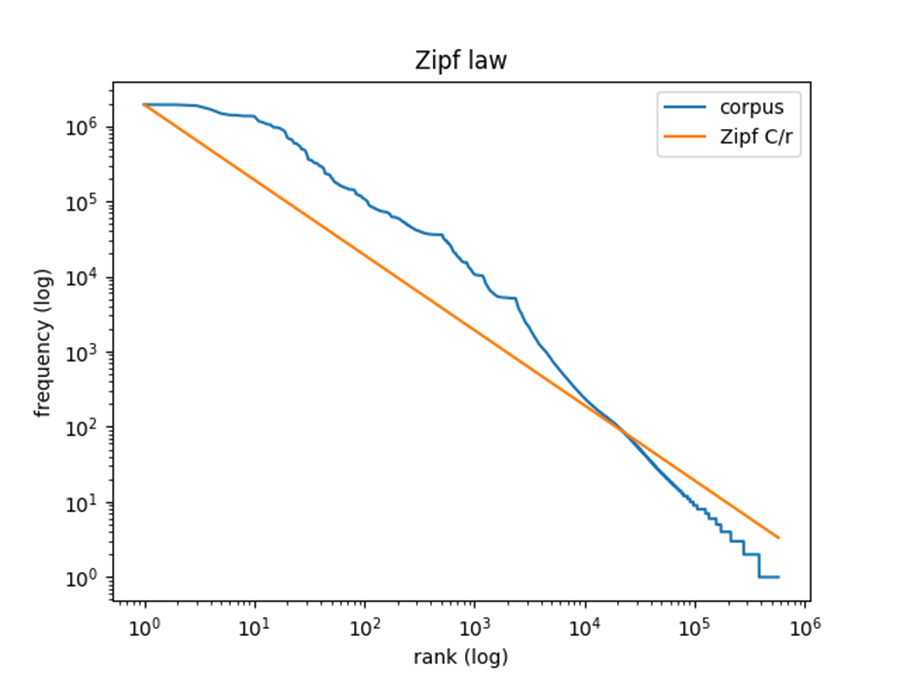
\includegraphics[width=0.8\linewidth]{images/zipf.png}
  \label{fig:my_image}
\end{figure}

\subsubsection*{3.5. Лемматизация / стемминг}

Для нормализации словоформ используется упрощённый стеммер (поддержка русского и английского). Нормализация применяется на этапе индексации и на этапе обработки запроса. 
\newline
Оценка качества: сравнение выдачи до/после стемминга на нескольких запросах, включая случаи ухудшения (омонимия, чрезмерное обрезание суффиксов).

\subsubsection*{3.6. Булев индекс}

Булев (инвертированный) индекс хранит для каждого термина список идентификаторов документов, в которых он встречается. Для словаря и списков документов используются собственные структуры данных (без map/unordered\_map).


\subsubsection*{3.7. Булев поиск и интерфейсы}

Поддерживаются операции AND, OR, NOT и круглые скобки. Результат поиска — список документов (url и источник). Реализованы два интерфейса:

\begin{itemize}
\item CLI: запросы читаются из stdin, результаты выводятся в stdout.
\item Web: HTTP-сервер с HTML-формой ввода и HTML-выдачей (на базе cpp-httplib).
\end{itemize}
\subsection*{4. Примеры запросов и проверка работы}

\subsubsection*{4.1. CLI}

Пример запуска CLI-поиска (индекс должен быть построен заранее):

\begin{lstlisting}[language=bash]
docker compose run --rm search /app/search_cli --index /data/index.bin
# stdin:
docker AND kubernetes
\end{lstlisting}

\subsubsection*{4.2. Web}

Пример запуска веб-сервиса:

\begin{lstlisting}[language=bash]
docker compose up -d search
# go to http://localhost:8080 in browser
\end{lstlisting}
\newline
Примеры запросов для проверки:

\begin{itemize}
\item docker AND compose
\item kubernetes OR helm
\item NOT windows
\item (python OR rust) AND (parser OR html)
\end{itemize}

\begin{figure}[ht]
  \centering
  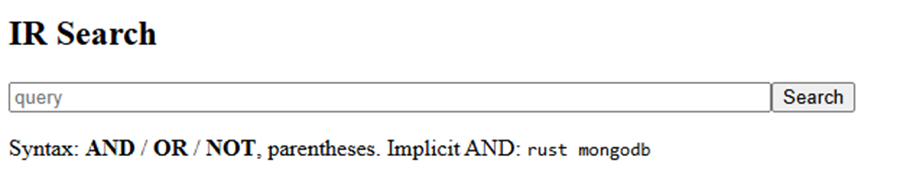
\includegraphics[width=0.8\linewidth]{images/ui_1.png}
  \label{fig:my_image}
\end{figure}

\begin{figure}[ht]
  \centering
  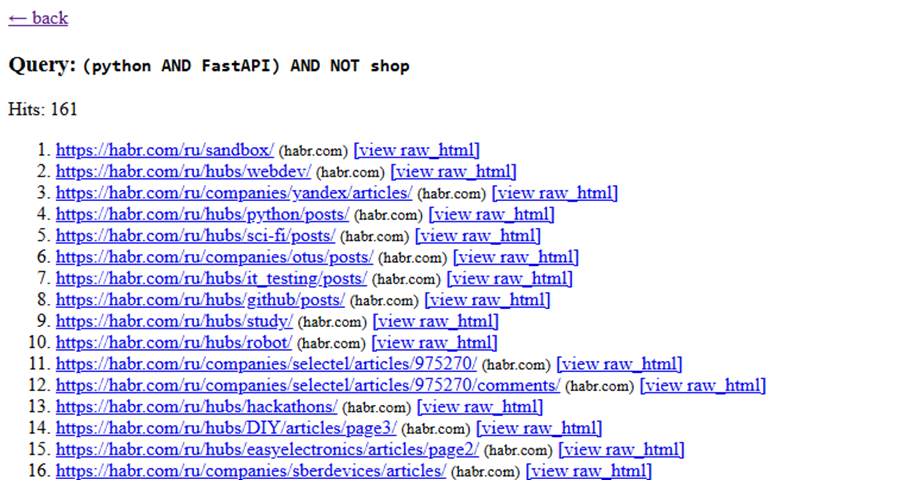
\includegraphics[width=0.8\linewidth]{images/ui_2.png}
  \label{fig:my_image}
\end{figure}

\begin{figure}[ht]
  \centering
  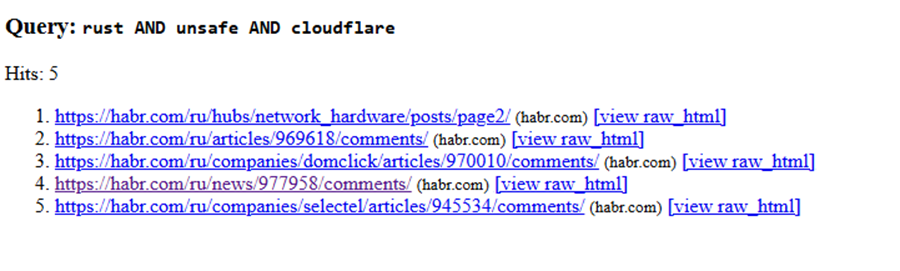
\includegraphics[width=0.8\linewidth]{images/ui_3.png}
  \label{fig:my_image}
\end{figure}

\subsection*{9. Итоговые выводы}

В ходе выполнения данных лабораторных работ я познакомился с тем, как устроены современные поисковые системы, и даже сумел реализовать свою собственную. 
\newline
Моя поисковая система:
\begin{itemize}
\item содержит расширяемый бинарный индекс, включающий обратный и прямой индексы, пригодный для булева поиска.
\item реализует булев поиск с поддержкой AND, OR, NOT, пробелов и скобок; 
\item запускается в Docker
\item предоставляет два интерфейса – CLI и Web
\item предоставляет возможность смотреть на raw HTML выдаваемых документов
\end{itemize}
\newline
Скорость выполнения запросов находится в миллисекундном диапазоне для типовых случаев; длительная работа возникает на выражениях с большими объединениями и отрицаниями частых термов.
\newline
В целом поисковую систему можно дорабатывать и приделывать к ней новые функции, которые позволят улучшить качество и скорость поиска

\end{document}